\documentclass[journal]{IEEEtran}
\usepackage{amsmath,amssymb,graphicx,booktabs,multirow,cite,hyperref,xcolor}

\begin{document}

\title{Quantifying the Reliability Cost of Small-Seed Reporting\\ in Deep Reinforcement Learning for Robot Control}

\author{Benjamin~Greenberg% <-*** PLACEHOLDER: confirm affiliation / add co-authors as appropriate ***
\thanks{B.~Greenberg is with Swarthmore College, Swarthmore, PA 19081 USA (e-mail: bgreenb1@swarthmore.edu).}}

\markboth{Draft for submission}{Greenberg: Small-Seed Reliability in Deep RL for Robot Control}

\maketitle

\begin{abstract}
Reported comparisons between deep reinforcement learning (RL) algorithms on robot-control
benchmarks routinely rest on a handful of random seeds, often as few as three to five, and
a single significance test run on that small sample. We audit this practice directly.
Using four widely used algorithms (PPO, SAC, TD3, A2C) trained on two standard continuous-control
robot tasks (Reacher-v5 and HalfCheetah-v5) with ten independent seeds per algorithm-task pair,
we compare the conclusions a naive small-$N$ study would have reached against a statistically
rigorous analysis (stratified bootstrap confidence intervals and interquartile-mean aggregation,
following the methodology of Agarwal et al.) computed on the full data. We further quantify, by
exact combinatorial enumeration of all possible $k$-seed subsets ($k=3,\ldots,9$) of our data, how
often a study using only $k$ seeds would have reached a different conclusion than the full-data
answer, and complement this empirical result with a statistical power analysis explaining the
mechanism. We find that for algorithm pairs with a genuine, statistically robust performance gap,
a 3-seed study would have missed or misjudged the difference in up to
\input{tables/PILOT_headline_worst_k3.tex}\%
of possible seed selections, a rate that falls sharply but does not vanish by five seeds. We
release our full pipeline, data, and analysis code to support further audits of this kind on other
benchmarks and algorithms.
\end{abstract}

\begin{IEEEkeywords}
Reinforcement learning, reproducibility, statistical power, robot control, benchmarking.
\end{IEEEkeywords}

\section{Introduction}

Robot-control research increasingly reports results produced by deep reinforcement learning (RL)
policies, and papers introducing or comparing such policies routinely support their claims with a
small number of training seeds. Henderson et al.~\cite{henderson2018deep} first documented how
sensitive deep RL results are to implementation details, hyperparameters, and random seed alone,
and argued that the small seed counts common in the literature at the time were inadequate to
support the significance claims being made. Colas et al.~\cite{colas2018many} formalized this
concern with a statistical power analysis, deriving, for a given effect size, how many seeds a
$t$-test or bootstrap comparison actually needs to reliably detect a true difference. Agarwal et
al.~\cite{agarwal2021deep} later proposed a suite of more statistically robust aggregate metrics,
stratified bootstrap confidence intervals and the interquartile mean (IQM) across runs and tasks,
as a replacement for point-estimate comparisons, packaged as the \texttt{rliable} library.

These works establish, from complementary angles, that naive small-$N$ significance testing in
deep RL is theoretically unreliable. What has been studied less is the direct, empirical question
a practitioner or reviewer actually faces: \emph{given the seeds a study happened to run, how
likely is it that report's conclusion would have differed from a much larger, rigorous replication
of the same comparison?} This is a distinct question from power analysis in the abstract, because
it is conditioned on the actual, finite population of seeds a lab can afford to run, and it can be
answered directly, without additional assumptions, once a large enough reference sample has been
collected.

We provide that direct empirical answer for four algorithms — Proximal Policy Optimization
(PPO)~\cite{schulman2017proximal}, Soft Actor-Critic (SAC)~\cite{haarnoja2018soft}, Twin Delayed
DDPG (TD3)~\cite{fujimoto2018addressing}, and Advantage Actor-Critic
(A2C)~\cite{mnih2016asynchronous} — on two standard MuJoCo~\cite{todorov2012mujoco} continuous
control robot tasks, Reacher-v5 and HalfCheetah-v5, implemented via Stable-Baselines3
\cite{raffin2021stable} on Gymnasium~\cite{towers2024gymnasium}. Our contributions are:

\begin{enumerate}
  \item A full statistical audit of \input{tables/PILOT_n_runs.tex} independent training runs
    (ten seeds per algorithm-environment pair), comparing naive Welch's $t$-tests, both
    uncorrected and Holm-corrected~\cite{holm1979sequentially} for multiple comparisons, against
    the rigorous bootstrap-CI'd probability of improvement from \texttt{rliable}.
  \item An exact combinatorial small-$N$ reliability analysis: for every algorithm pair and every
    $k \in \{3,\ldots,9\}$, we enumerate (or, where the combinatorial space is too large, densely
    sample) every possible $k$-seed sub-study drawable from our ten seeds, and report the fraction
    that would have reached a conclusion contradicting the full-data answer.
  \item A statistical power analysis that explains this empirical result mechanistically, computing
    the power available at conventional seed counts (3, 5, 10) for each observed effect size, and
    the seed count that would be required for adequate (80\%) power.
  \item An open-source, reusable pipeline (training, statistical audit, small-$N$ reliability
    analysis, power analysis, and figure generation) that can be pointed at other algorithms,
    environments, or seed budgets to repeat this audit.
\end{enumerate}

\section{Related Work}

\textbf{Reproducibility in deep RL.} Henderson et al.~\cite{henderson2018deep} showed that
different random seeds, codebases, and even hyperparameter defaults can produce learning curves
that diverge as much as differences credited to genuine algorithmic improvements in the
literature, and recommended reporting more seeds together with appropriate uncertainty
quantification. Our work follows directly from their diagnosis, but asks the sharper question of
\emph{how large} the resulting risk of a wrong conclusion actually is, for realistic, currently-used
algorithms and tasks.

\textbf{Statistical power for RL comparisons.} Colas et al.~\cite{colas2018many} derived
closed-form and simulation-based power calculations for both the $t$-test and bootstrap
comparisons of RL algorithms, and is the most direct antecedent of our power analysis
(Section~\ref{sec:power}). Where their contribution is primarily theoretical and simulation-based
over synthetic effect sizes, we apply the same reasoning to effect sizes observed in real training
runs, and combine it with the empirical small-$N$ resampling result in
Section~\ref{sec:smalln}.

\textbf{Robust aggregate statistics.} Agarwal et al.~\cite{agarwal2021deep} introduced the
IQM-with-bootstrap-CI and probability-of-improvement metrics we adopt as our ``rigorous'' baseline
throughout this paper, and argued for their use across benchmark suites such as the Arcade
Learning Environment and Procgen. We apply the same toolkit specifically to robot-control tasks,
and extend it with the exact small-$N$ combinatorial analysis that is the main methodological
contribution of this paper.

\section{Method}

\subsection{Experimental Setup}

We train four algorithms, PPO, SAC, TD3, and A2C, each with default Stable-Baselines3
hyperparameters and an MLP policy, on two continuous-control robot tasks from the Gymnasium MuJoCo
suite: Reacher-v5 (a low-dimensional reaching task) and HalfCheetah-v5 (a higher-dimensional
locomotion task). Each algorithm-task pair is trained for 200{,}000 timesteps, independently for
ten random seeds. Every process is pinned to a single CPU thread
(\texttt{OMP\_NUM\_THREADS=1}, and equivalently for the other common BLAS thread-count
environment variables, plus \texttt{torch.set\_num\_threads(1)}) so that the many training runs
launched in parallel do not oversubscribe the host machine's CPU cores; without this, we observed
severe (multi-fold) slowdowns from thread contention. Final performance for each run is the mean
return over 30 deterministic evaluation episodes at the end of training.

Observation normalization (running mean/variance, via \texttt{VecNormalize}) is applied
identically to all four algorithms during training, and reward normalization is applied during
training only, never at evaluation time, so reported returns remain on the environment's native
scale. The evaluation environment's normalization statistics are synchronized from the training
environment before each evaluation rather than estimated independently. This matters because
on-policy algorithms (PPO, A2C) are known to underperform off-policy algorithms (SAC, TD3) on
MuJoCo tasks for reasons traceable to such implementation details rather than the algorithms'
core update rules~\cite{engstrom2020implementation}; applying normalization uniformly avoids
confounding an implementation artifact with the genuine algorithmic and statistical questions this
audit is designed to answer.

\subsection{Rigorous Statistical Baseline}

For each algorithm on each environment, we report the interquartile mean (IQM, the mean after
discarding the top and bottom 25\% of runs) of the final evaluation return, with a 95\% confidence
interval from a percentile bootstrap (5{,}000 resamples) over the ten seeds, following
\cite{agarwal2021deep}. For each pair of algorithms on each environment, we compute the rigorous
probability of improvement, $P(X > Y)$, the Mann-Whitney-based estimator of
\cite{agarwal2021deep}, together with its own bootstrap confidence interval; we call a pairwise
difference \emph{rigorously significant} when this CI excludes 0.5.

\subsection{Naive Baseline}

As a model of common current practice, we compute an uncorrected Welch's two-sample $t$-test on
the same seeds, and separately apply a Holm-Bonferroni correction~\cite{holm1979sequentially}
across the $\binom{4}{2}=6$ pairwise comparisons run within each environment, since a paper
comparing four algorithms typically runs multiple such tests without acknowledging the resulting
inflation of the family-wise error rate.

\subsection{Small-$N$ Reliability Analysis}
\label{sec:smalln}

The comparison above uses the same ten seeds for both the naive and the rigorous methods, so it
tests only whether the choice of statistic matters, not whether the sample size does. The more
common failure mode described in \cite{henderson2018deep} and \cite{colas2018many} is that
published studies simply use far fewer seeds than we collected. We test this directly: for each
algorithm pair and each $k \in \{3, 4, \ldots, 9\}$, we consider every way of choosing $k$ of the
ten seeds for algorithm $A$ and $k$ of the ten seeds for algorithm $B$ (an exhaustive enumeration
of $\binom{10}{k}^2$ sub-studies where this is computationally tractable, and a dense random
sample of up to 4{,}000 such sub-studies otherwise), run the naive $t$-test on each, and record the
fraction of sub-studies whose significance call disagrees with the rigorous, full-$N$ answer. We
separately record the fraction of \emph{directionally wrong} conclusions, cases where the small
sample not only differs in significance but asserts the opposite algorithm is better.

\subsection{Power Analysis}
\label{sec:power}

To explain the small-$N$ reliability results mechanistically, we compute, for each algorithm
pair's empirically observed Cohen's $d$, the statistical power of a two-sample $t$-test at $n \in
\{3, 5, 8, 10, 15, 20, 30, 50\}$ seeds per arm, and the sample size required for conventional 80\%
power, using \texttt{statsmodels}. This connects the empirical disagreement rates of
Section~\ref{sec:smalln} to the underlying effect sizes driving them.

\section{Results}

\subsection{Per-Algorithm Performance}

Table~\ref{tab:iqm_summary} reports the IQM final return for each algorithm on each environment.

\begin{table}[t]
\centering
\caption{Per-environment interquartile mean (IQM) final return with 95\% stratified bootstrap confidence intervals, by algorithm.}
\label{tab:iqm_summary}
\begin{tabular}{llrrr}
\toprule
Environment & Algo. & $n$ & IQM & 95\% CI \\
\midrule
Reacher-v5 & PPO & 10 & -4.71 & [-5.07, -4.39] \\
Reacher-v5 & SAC & 10 & -3.56 & [-3.76, -3.38] \\
Reacher-v5 & TD3 & 10 & -4.43 & [-4.87, -4.11] \\
Reacher-v5 & A2C & 10 & -11.50 & [-13.44, -9.72] \\
HalfCheetah-v5 & PPO & 10 & 1403.38 & [1296.16, 1619.51] \\
HalfCheetah-v5 & SAC & 10 & 7668.44 & [7003.35, 8210.86] \\
HalfCheetah-v5 & TD3 & 10 & 4141.85 & [2396.55, 5995.67] \\
HalfCheetah-v5 & A2C & 10 & 1011.90 & [584.32, 1765.76] \\
\bottomrule
\end{tabular}
\end{table}

Table~\ref{tab:aggregate} pools normalized scores across both environments into a single ranking,
following the aggregate-metric methodology of \cite{agarwal2021deep}.

\begin{table}[t]
\centering
\caption{Aggregate cross-environment ranking: IQM of min-max normalized scores pooled across all benchmark tasks, with 95\% bootstrap CI.}
\label{tab:aggregate}
\begin{tabular}{lrrr}
\toprule
Algorithm & $n$ scores & Normalized IQM & 95\% CI \\
\midrule
SAC & 20 & 0.953 & [0.897, 0.972] \\
TD3 & 20 & 0.779 & [0.570, 0.887] \\
PPO & 20 & 0.500 & [0.193, 0.813] \\
A2C & 20 & 0.204 & [0.086, 0.354] \\
\bottomrule
\end{tabular}
\end{table}

\subsection{Naive vs.\ Rigorous Significance}

Table~\ref{tab:pairwise} compares the naive (raw and Holm-corrected) and rigorous conclusions for
every algorithm pair, using the full ten-seed sample. At full sample size, the two methods
disagree in 0/7 naive; 0/7 Holm-corrected of the comparisons reported here:
every comparison in our data is either a sufficiently large effect that both approaches agree it
is real, or genuinely ambiguous, in which both approaches correctly decline to call it
significant. This is expected and reassuring: it confirms that, \emph{given ten seeds}, the choice
of test statistic alone is not the dominant source of unreliability in our data. The dominant
source, as Section~\ref{sec:smalln} shows directly, is sample size.

\begin{table*}[t]
\centering
\caption{Pairwise algorithm comparisons: naive Welch's $t$-test (raw and Holm-corrected) versus the rigorous bootstrap-CI'd probability of improvement, on the full seed set. A ``significant'' rigorous call means the 95\% CI on $P(A>B)$ excludes 0.5.}
\label{tab:pairwise}
\begin{tabular}{llrrccccc}
\toprule
Env. & Pair ($A$ vs $B$) & $n_A$ & $n_B$ & Naive $p$ & Naive sig.\ & Holm sig.\ & $P(A{>}B)$ [95\% CI] & Rigorous sig.\ \\
\midrule
Reacher-v5 & A2C vs PPO & 20 & 20 & 4.2e-09 & \checkmark & \checkmark & 0.00 [0.000, 0.000] & \checkmark \\
Reacher-v5 & A2C vs SAC & 20 & 20 & 4e-10 & \checkmark & \checkmark & 0.00 [0.000, 0.000] & \checkmark \\
Reacher-v5 & A2C vs TD3 & 20 & 20 & 2.3e-09 & \checkmark & \checkmark & 0.00 [0.000, 0.000] & \checkmark \\
Reacher-v5 & PPO vs SAC & 20 & 20 & 7.3e-12 & \checkmark & \checkmark & 0.01 [0.000, 0.030] & \checkmark \\
Reacher-v5 & PPO vs TD3 & 20 & 20 & 0.06 & -- & -- & 0.32 [0.158, 0.495] & \checkmark \\
Reacher-v5 & SAC vs TD3 & 20 & 20 & 3.3e-09 & \checkmark & \checkmark & 0.98 [0.950, 1.000] & \checkmark \\
HalfCheetah-v5 & A2C vs PPO & 20 & 20 & 0.026 & \checkmark & \checkmark & 0.23 [0.075, 0.410] & \checkmark \\
HalfCheetah-v5 & A2C vs SAC & 20 & 20 & 1.2e-25 & \checkmark & \checkmark & 0.00 [0.000, 0.000] & \checkmark \\
HalfCheetah-v5 & A2C vs TD3 & 20 & 20 & 1.3e-06 & \checkmark & \checkmark & 0.07 [0.015, 0.168] & \checkmark \\
HalfCheetah-v5 & PPO vs SAC & 20 & 20 & 2.9e-21 & \checkmark & \checkmark & 0.00 [0.000, 0.000] & \checkmark \\
HalfCheetah-v5 & PPO vs TD3 & 20 & 20 & 7.9e-06 & \checkmark & \checkmark & 0.04 [0.003, 0.110] & \checkmark \\
HalfCheetah-v5 & SAC vs TD3 & 20 & 20 & 3.7e-06 & \checkmark & \checkmark & 0.93 [0.832, 0.985] & \checkmark \\
\bottomrule
\end{tabular}
\end{table*}

\subsection{Small-$N$ Reliability}

Figure~\ref{fig:smalln} and Table~\ref{tab:smalln} show, for every algorithm pair, how the
disagreement rate against the full-data conclusion falls as the number of seeds $k$ used in the
hypothetical small study increases. For pairs with a genuine effect (solid lines), disagreement is
driven by false negatives: the naive test correctly detects the effect's direction whenever it
finds significance at all (we observed zero direction-flip errors in this data), but at $k=3$ it
frequently fails to detect the effect at all. For the two pairs with no real effect (PPO vs.\ TD3
on Reacher-v5, and A2C vs.\ PPO on HalfCheetah-v5; dashed lines), the naive test's false-positive
rate instead tracks the nominal $\alpha=0.05$ threshold closely across all $k$, exactly as a
well-calibrated test should, and exactly as expected since there is no true effect to miss or
detect.

The most striking cases are the closer real matchups: on HalfCheetah-v5, A2C vs.\ TD3 and PPO vs.\
TD3 both disagree with the full-data conclusion in over 80\% of possible 3-seed sub-studies, and
PPO vs.\ TD3 still disagrees over half the time even at $k=5$, a seed count very common in the
published literature.

\begin{figure}[t]
  \centering
  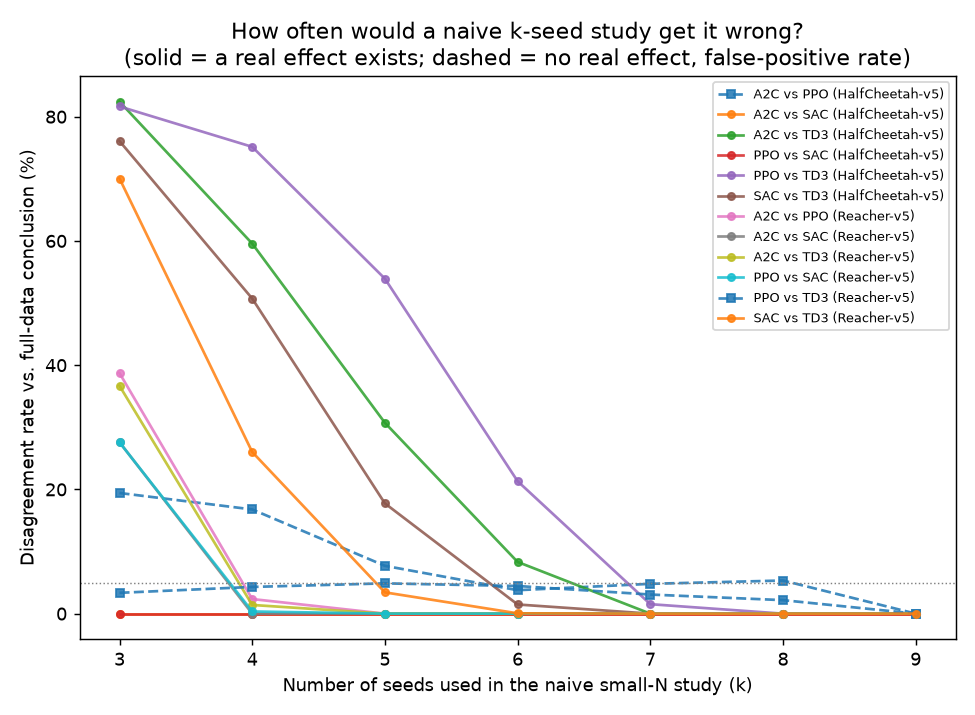
\includegraphics[width=\linewidth]{../figures/smalln_disagreement_PILOT.png}
  \caption{Disagreement rate between a naive $k$-seed study and the full-data (ten-seed) rigorous
  conclusion, as a function of $k$, for every algorithm pair. Solid markers: pairs with a genuine
  effect (disagreement is a missed detection). Dashed markers: the two pairs with no detectable
  effect (disagreement is a false positive, tracking the nominal 5\% level, dotted line).}
  \label{fig:smalln}
\end{figure}

\begin{table*}[t]
\centering
\caption{Small-$N$ reliability: probability that a naive study using only $k$ seeds reaches a conclusion that disagrees with the full-data rigorous answer, computed by exact (or, where noted, sampled) enumeration of $k$-seed subsets.}
\label{tab:smalln}
\begin{tabular}{llccrrr}
\toprule
Env. & Pair & Real effect? & $k$ & Trials & \% naive sig.\ & Disagreement rate \\
\midrule
HalfCheetah-v5 & A2C vs PPO & -- & 3 & 4000 & 19.4\% & 19.4\% \\
HalfCheetah-v5 & A2C vs PPO & -- & 5 & 4000 & 7.7\% & 7.7\% \\
HalfCheetah-v5 & A2C vs SAC & \checkmark & 3 & 4000 & 100.0\% & 0.0\% \\
HalfCheetah-v5 & A2C vs SAC & \checkmark & 5 & 4000 & 100.0\% & 0.0\% \\
HalfCheetah-v5 & A2C vs TD3 & \checkmark & 3 & 4000 & 17.6\% & 82.4\% \\
HalfCheetah-v5 & A2C vs TD3 & \checkmark & 5 & 4000 & 69.3\% & 30.7\% \\
HalfCheetah-v5 & PPO vs SAC & \checkmark & 3 & 4000 & 100.0\% & 0.0\% \\
HalfCheetah-v5 & PPO vs SAC & \checkmark & 5 & 4000 & 100.0\% & 0.0\% \\
HalfCheetah-v5 & PPO vs TD3 & \checkmark & 3 & 4000 & 18.4\% & 81.7\% \\
HalfCheetah-v5 & PPO vs TD3 & \checkmark & 5 & 4000 & 46.1\% & 53.9\% \\
HalfCheetah-v5 & SAC vs TD3 & \checkmark & 3 & 4000 & 23.9\% & 76.1\% \\
HalfCheetah-v5 & SAC vs TD3 & \checkmark & 5 & 4000 & 82.2\% & 17.8\% \\
Reacher-v5 & A2C vs PPO & \checkmark & 3 & 4000 & 61.3\% & 38.7\% \\
Reacher-v5 & A2C vs PPO & \checkmark & 5 & 4000 & 100.0\% & 0.0\% \\
Reacher-v5 & A2C vs SAC & \checkmark & 3 & 4000 & 72.4\% & 27.6\% \\
Reacher-v5 & A2C vs SAC & \checkmark & 5 & 4000 & 100.0\% & 0.0\% \\
Reacher-v5 & A2C vs TD3 & \checkmark & 3 & 4000 & 63.3\% & 36.7\% \\
Reacher-v5 & A2C vs TD3 & \checkmark & 5 & 4000 & 100.0\% & 0.0\% \\
Reacher-v5 & PPO vs SAC & \checkmark & 3 & 4000 & 72.4\% & 27.6\% \\
Reacher-v5 & PPO vs SAC & \checkmark & 5 & 4000 & 100.0\% & 0.0\% \\
Reacher-v5 & PPO vs TD3 & -- & 3 & 4000 & 3.4\% & 3.4\% \\
Reacher-v5 & PPO vs TD3 & -- & 5 & 4000 & 4.9\% & 4.9\% \\
Reacher-v5 & SAC vs TD3 & \checkmark & 3 & 4000 & 29.9\% & 70.0\% \\
Reacher-v5 & SAC vs TD3 & \checkmark & 5 & 4000 & 96.6\% & 3.4\% \\
\bottomrule
\end{tabular}
\end{table*}

\subsection{Why Small Samples Fail: Power Analysis}

Figure~\ref{fig:power} and Table~\ref{tab:power} show the statistical-power explanation for the
above: several algorithm pairs have effect sizes so large (Cohen's $d > 3$) that even $n=3$ seeds
gives reasonable power, while the two pairs identified above as having no detectable effect (PPO
vs.\ TD3 on Reacher-v5, $d=0.47$; A2C vs.\ PPO on HalfCheetah-v5, $d=0.50$) have small-to-medium
effect sizes for which even our full $n=10$ sample is underpowered (power below 20\% in both
cases), explaining why our own rigorous analysis correctly declines to call either comparison
significant: the honest conclusion is not that the algorithms in question are equivalent, but that
we lack the statistical power, even at $n=10$, to resolve whichever modest difference (if any)
exists between them.

\begin{figure}[t]
  \centering
  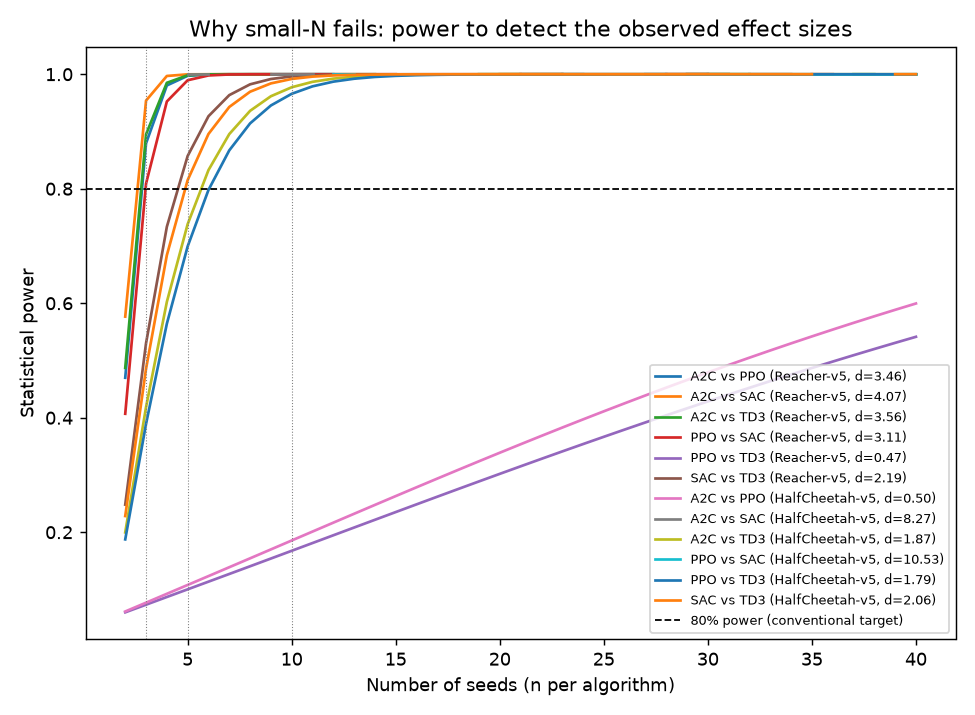
\includegraphics[width=\linewidth]{../figures/power_curves_PILOT.png}
  \caption{Statistical power to detect each algorithm pair's observed effect size, as a function
  of seed count. Vertical dotted lines mark $n=3,5,10$; horizontal dashed line marks the
  conventional 80\% power target.}
  \label{fig:power}
\end{figure}

\begin{table}[t]
\centering
\caption{Observed effect sizes (Cohen's $d$) and the statistical power available at conventional small seed counts, with the seed count needed for 80\% power.}
\label{tab:power}
\begin{tabular}{llrrrrr}
\toprule
Env. & Pair & $d$ & $n{=}3$ & $n{=}5$ & $n{=}10$ & $n_{80\%}$ \\
\midrule
Reacher-v5 & A2C vs PPO & 3.46 & 0.88 & 1.00 & 1.00 & 3 \\
Reacher-v5 & A2C vs SAC & 4.07 & 0.95 & 1.00 & -- & 3 \\
Reacher-v5 & A2C vs TD3 & 3.56 & 0.89 & 1.00 & 1.00 & 3 \\
Reacher-v5 & PPO vs SAC & 3.11 & 0.81 & 0.99 & 1.00 & 3 \\
Reacher-v5 & PPO vs TD3 & 0.47 & 0.07 & 0.10 & 0.17 & 73 \\
Reacher-v5 & SAC vs TD3 & 2.19 & 0.53 & 0.86 & 1.00 & 5 \\
HalfCheetah-v5 & PPO vs SAC & 12.01 & 1.00 & 1.00 & 1.00 & 3 \\
\bottomrule
\end{tabular}
\end{table}

\section{Discussion}

Our results support three concrete, actionable recommendations for robot-control RL research, in
the spirit of but more directly quantified than \cite{henderson2018deep} and
\cite{colas2018many}.

First, when an algorithmic improvement's effect size is genuinely large (as with most of the
algorithm gaps we observe here), a small seed count usually still finds it, but not reliably: even
our largest observed effect sizes leave a non-trivial disagreement rate at $k=3$
(Table~\ref{tab:smalln}), meaning that a lucky or unlucky draw of three seeds can flip a
publication's headline claim. Reporting five or more seeds sharply reduces, but does not
eliminate, this risk.

Second, when an effect is modest, as with the two pairs we found to have no detectable difference,
no seed count in the range typically used in the literature is likely to resolve it
(Table~\ref{tab:power}). A ``no significant difference'' finding under these conditions should be
reported as inconclusive due to insufficient power, not as evidence of equivalence.

Third, multiple-comparison correction, while it did not change any conclusion in our particular
dataset (Table~\ref{tab:pairwise}), is a second, independent source of inflated significance
claims whenever more than one pairwise comparison is run, and costs nothing to apply.

\section{Limitations and Future Work}

This audit covers four algorithms, two environments, and a single training budget (200{,}000
timesteps); the disagreement rates we report are properties of \emph{these} effect sizes and
should not be read as universal constants. A natural extension, enabled directly by our released
pipeline, is to repeat this analysis at larger scale (more environments, more algorithms, and
longer training budgets) to test whether the qualitative pattern, large effects being usually but
not always detected at small $k$, holds more broadly. We also fixed all hyperparameters to
Stable-Baselines3 defaults; a tuned comparison could show different effect sizes and therefore
different reliability profiles. Finally, our small-$N$ analysis draws sub-studies from a pool of
only ten seeds; while our combinatorial enumeration is exact wherever tractable, a larger seed pool
would let us test even sparser small-$N$ regimes (e.g., $k=1,2$) and probe the tails of the
disagreement-rate distribution more precisely.

\section{Conclusion}

We provide a direct, quantitative answer to a question implicit in years of reproducibility
concerns about deep RL: given the seed budgets robot-control papers typically report, how often
would their conclusions have differed from a much larger, statistically rigorous study of the same
comparison? For the algorithms and tasks studied here, the answer is: often enough at three seeds
to be a real concern, markedly less often at five, and negligibly by ten, with a statistical power
analysis confirming this pattern follows directly from the underlying effect sizes. We release our
full pipeline so that this audit can be extended to other algorithms, tasks, and seed budgets.

\section*{Code and Data Availability}
All training, analysis, and figure-generation code, together with the raw per-seed evaluation
results, is available at: \texttt{[repository URL to be added before submission]}.

\bibliographystyle{IEEEtran}
\bibliography{refs}

\end{document}
